% =========================================================================
% CAPITOLO 3 — RASSEGNA DELLA LETTERATURA
% =========================================================================

\chapter{Rassegna della letteratura}
\label{ch:literature}


\noindent
{\rmfamily\itshape
\begin{tabular}[t]{@{}l@{\hspace{0.3cm}}p{12.5cm}@{}}
\textls[50]{\textbf{Trattati:}} &
\textls[50]{Fondamenti teorici · Percezione del rischio e limiti cognitivi · Benchmark attuali ·
Rappresentazione incarnata e immersiva · Principi di design · Vuoti nella letteratura}
\end{tabular}
}

\vspace{0.5cm}

Questo capitolo esamina la letteratura su cui la tesi è costruita. Tre filoni definiscono il problema: la psicologia della percezione del rischio climatico, la scienza cognitiva dei sistemi dinamici e la valutazione empirica della visualizzazione del clima. Due forniscono la risposta: la rappresentazione incarnata e immersiva, e il machine learning usato in modo rappresentativo anziché predittivo. Un sesto filone traduce la teoria in una grammatica di design, e una sezione conclusiva nomina il vuoto che la tesi occupa.

% -------------------------------------------------------------------------
\section{Barriere psicologiche alla percezione del rischio climatico}
\label{sec:psych-barriers}

Il Capitolo~\ref{ch:introduction} ha introdotto l'\emph{ipotesi del deficit di informazione} e l'evidenza contraria \citep{kellstedt2008, kahan2015}.\footnote{In \citet{kellstedt2008} la relazione inversa tra conoscenza e preoccupazione è sopravvissuta ai controlli per affiliazione politica e fattori demografici, indicando un genuino effetto cognitivo-culturale anziché un fattore confondente.} Ciò che conta qui è \emph{perché} fallisce, perché è a questo che il design deve rispondere: l'informazione conta, ma il suo effetto è mediato da meccanismi cognitivi e culturali che i formati standard non hanno mai affrontato.

Il resoconto più influente di questo fallimento è \citet{stoknes2015}, che nomina cinque barriere --- \emph{distanza}, \emph{catastrofismo}, \emph{dissonanza}, \emph{negazione} e \emph{identità} --- che hanno organizzato gran parte del lavoro successivo.\footnote{In breve: \emph{distanza} (il cambiamento climatico appare spazialmente, temporalmente e socialmente remoto), \emph{catastrofismo} (l'inquadramento catastrofista innesca l'evitamento), \emph{dissonanza} (il divario credenza--comportamento si risolve aggiustando la credenza), \emph{negazione} (disimpegno autoprotettivo) e \emph{identità} (le posizioni sul clima segnalano l'appartenenza a un gruppo).} Le barriere si intrecciano anziché agire singolarmente \citep{vanderlinden2015}, e il pubblico si stratifica in gruppi le cui barriere si attivano in modo diverso, perciò nessuna singola strategia le serve tutte \citep{leiserowitz2021}. La visualizzazione convenzionale non le ha dissolte, e la ragione è strutturale: le immagini più usate per comunicare il cambiamento climatico o rafforzano la distanza che i comunicatori sperano di colmare o innescano la risposta di catastrofismo che sopprime il coinvolgimento \citep{cornerclimate2015, nicholsoncole2005}, e i formati che non danno al lettore alcun ruolo attivo rendono costantemente meno di quelli che glielo danno \citep{ojala2023}. Aggiungere precisione a un grafico a linee non apre alcun ruolo di questo tipo --- la sua retorica implicita del \emph{ecco il fatto} non lascia al lettore alcun punto su cui stare. La letteratura punta quindi verso rappresentazioni che trattano il lettore come partecipante attivo nella costruzione del significato \citep{marlon2019, morris2019}, che è la direzione che questa tesi persegue, con il machine learning come substrato.

% -------------------------------------------------------------------------
\section{La scienza cognitiva dei sistemi dinamici e complessi}
\label{sec:cognitive-science}

Sotto questi filtri culturali si trova una barriera indipendente da essi: i limiti strutturali della mente nel ragionare su sistemi di accumulo, retroazione e ritardo. Sono caratteristiche stabili dell'architettura cognitiva, non lacune che un insegnamento migliore potrebbe colmare, e qualsiasi rappresentazione che le ignori fallirà per quanto bene sia calibrata psicologicamente.

L'evidenza più forte è \citet{sterman2008}, i cui esperimenti mostrano che perfino adulti matematicamente competenti commettono errori sistematici su elementari problemi di stock e flusso. Mostrato uno scenario in cui la CO\textsubscript{2} atmosferica si stabilizza, e chiesto di tracciare il percorso delle emissioni coerente con esso, la maggior parte viola il bilancio di massa --- facendo corrispondere la forma dell'uscita a quella dell'ingresso anziché ragionare sulla differenza tra flusso in entrata e in uscita.
\footnote{Negli studi di Sterman l'84\% dei partecipanti molto istruiti --- dottorandi del MIT, ingegneri, partecipanti con formazione in analisi matematica --- ha commesso questo errore, indicando un limite di rappresentazione anziché di aritmetica.} \citet{cronin2009} ha trovato lo stesso in forma più netta: chiesto di tracciare uno stock dal suo flusso in entrata e in uscita, i partecipanti hanno confuso i tassi con i livelli e trattato il sistema dinamico come statico, anche quando possedevano l'apparato matematico per risolverlo. Dato solo un grafico, la mente non costruisce spontaneamente lo scenario dinamico che il grafico raffigura.

% it/figures/literature/sterman_figures.tex — versione italiana
\begin{figure}[htbp]
    \centering
    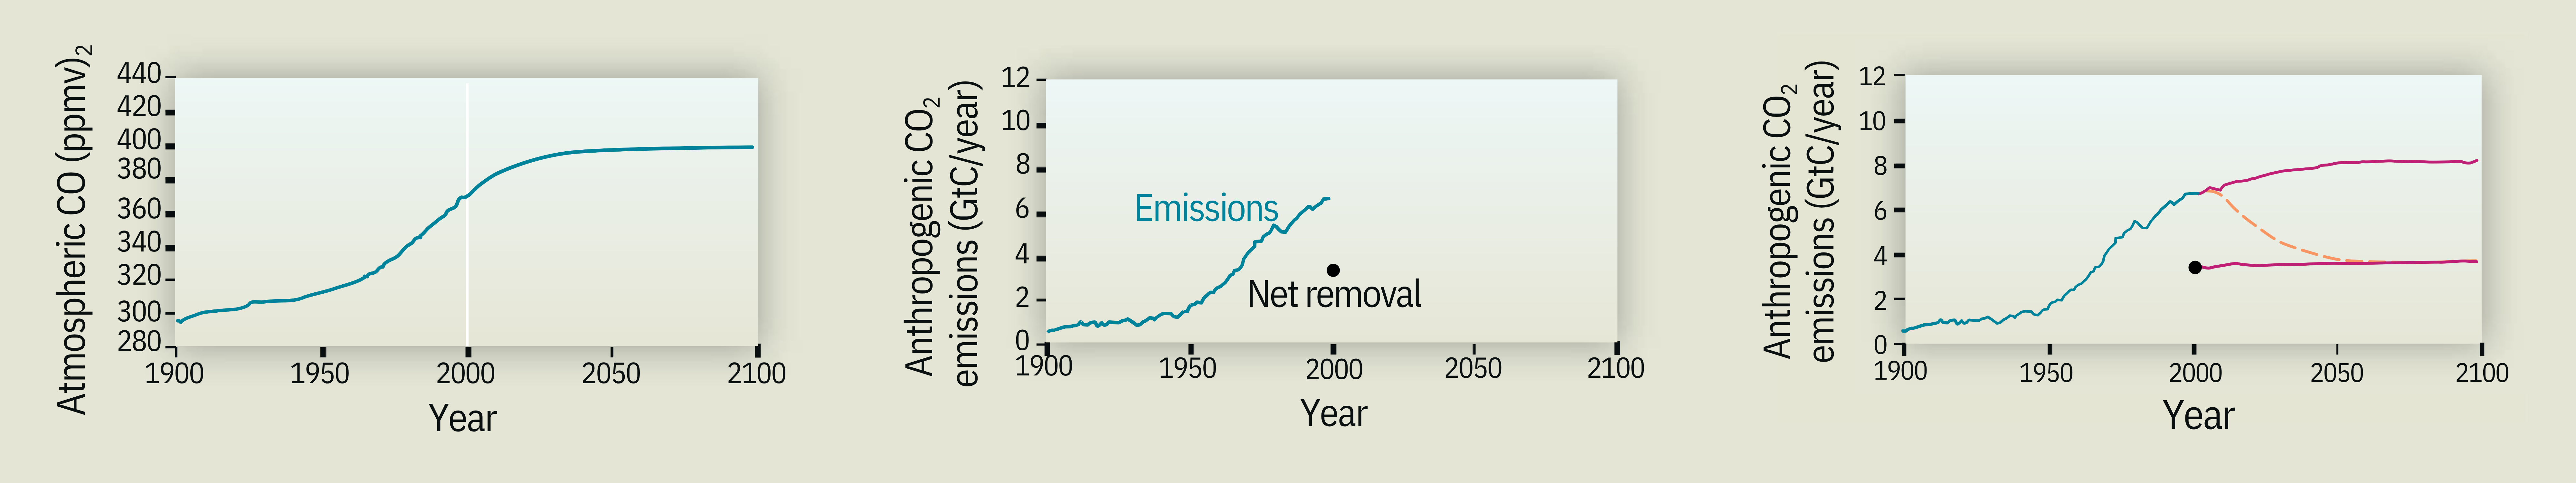
\includegraphics[width=\textwidth]{figures/literature/sterman_panel.png}
    \caption[Il compito di stabilizzazione del clima]{Il compito di stabilizzazione
    del clima. (a)~Lo scenario presentato ai partecipanti: la concentrazione
    atmosferica di CO\textsubscript{2} sale gradualmente a 400~ppmv e si stabilizza
    entro il 2100. (b)~L'informazione stock--flusso fornita: le emissioni antropiche
    di CO\textsubscript{2} dal 1900 al 2000 (il flusso in entrata) e l'attuale
    rimozione netta da parte di oceani e biomassa (il flusso in uscita), con le
    emissioni circa doppie rispetto alla rimozione netta. (c)~Una risposta tipica: i
    partecipanti disegnano erroneamente emissioni future che ricalcano la forma della
    traiettoria della CO\textsubscript{2} (euristica del pattern-matching), mentre il
    bilancio di massa richiede che le emissioni calino finché non eguagliano la
    rimozione netta (linea tratteggiata). Ristampato da \citet{sterman2008}.}
    \label{fig:sterman-panel}
\end{figure}


La teoria del carico cognitivo spiega perché \citep{sweller1988, swellervanmerrienboer2019}: la memoria di lavoro è strettamente limitata, e un'immagine statica di un sistema dinamico chiede al lettore di animare mentalmente ciò che l'immagine non anima --- un onere che si aggiunge al dominio stesso. \citet{ware2021} sostiene che una visualizzazione comunicativa deve abbassare questa richiesta di simulazione interna rendendo la struttura dinamica percettivamente disponibile. Un terzo filone guarda avanti: \citet{tversky2019}, sintetizzando quattro decenni di lavoro, mostra che ragionare su processi complessi è fondamentalmente spaziale, compreso attraverso schemi corporei e cinestesici. Se ragionare sulle dinamiche è spazialmente incarnato, le strategie con maggiori probabilità di successo arruolano la cognizione spaziale e cinestesica del lettore --- la proposizione che organizza il resto del capitolo.

% -------------------------------------------------------------------------
\section{Valutazione empirica della visualizzazione del clima}
\label{sec:empirical-viz}

Ciò che è stato misurato su come le visualizzazioni del clima vengono recepite rivela un'asimmetria metodologica: il campo è ricco di studi su ciò che il pubblico \emph{preferisce} e scarso di studi su ciò che \emph{comprende} --- il vuoto che questa tesi affronta. La rassegna più sistematica ha rilevato che i formati standard --- grafici a linee, mappe coropletiche, grafici spaghetti d'ensemble --- sono mal calibrati rispetto alle risorse cognitive del loro pubblico, anche tra lettori esperti di policy \citep{harold2016}. Mostrati un grafico di proiezione dell'IPCC, tali lettori vedono molta incertezza ma la attribuiscono ai modelli, trascurando l'incertezza di scenario che gli stessi intervalli contengono \parencite{mcmahon2015}. In modo più rivelatore, le visualizzazioni che le persone \emph{preferiscono} non sono quelle che producono la più alta \emph{comprensione}: le persone scelgono display più ricchi e realistici anche quando questi le rallentano e ne abbassano l'accuratezza \parencite{hegarty2012}. Ottimizzare per la preferenza rischia quindi di produrre ciò che \citet{sheppard2015} chiama \emph{visualizzazioni consolatorie} --- immagini accolte calorosamente e comprese male.

Questo poggia su una matura scienza della codifica visiva su cui il Capitolo~\ref{ch:translate} attinge direttamente. Bertin ha individuato l'insieme finito di \emph{variabili visive} attraverso cui qualsiasi segno codifica dati \citep{bertin1983}; \citet{clevelandmcgill1984} le ha ordinate per accuratezza di decodifica, con la posizione lungo una scala comune giudicata assai più accuratamente di lunghezza, angolo, area o colore; e \citet{munzner2014} ha trasformato questo nella regola di design dell'\emph{efficacia} --- assegnare l'informazione più importante al canale decodificato con maggiore accuratezza. \citet{ware2021} fonda la stessa regola nella percezione pre-attentiva. La codifica, in breve, è prestazione percettiva misurata, non gusto.

% it/figures/literature/cleveland_hierarchy.tex — versione italiana
\begin{figure}[!ht]
    \centering
    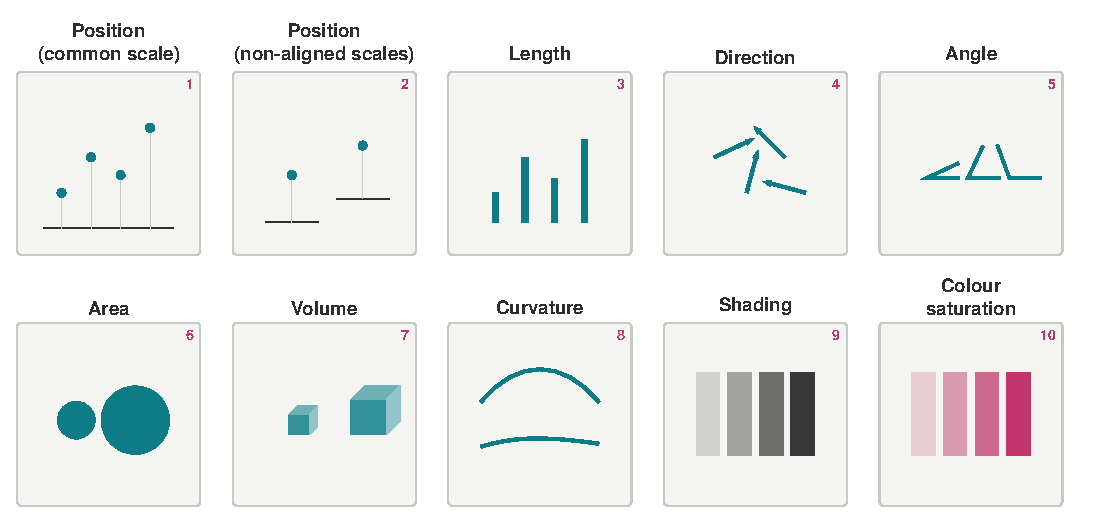
\includegraphics[width=\textwidth]{figures/literature/cleveland_preview.pdf}
    \caption[La gerarchia dei compiti percettivi di Cleveland \& McGill.]{\textbf{La
    gerarchia dei compiti percettivi elementari, secondo \citet{clevelandmcgill1984}.}
    Le codifiche sono ordinate per accuratezza di decodifica, dalla più accurata (1,
    posizione su una scala comune) alla meno accurata (10, saturazione del colore).
    L'ordinamento è empirico, non estetico: riflette quanto accuratamente le persone
    estraggono un valore quantitativo da ciascun canale visivo. Sta alla base del
    principio~P0 della grammatica di design (Tabella~\ref{tab:design-grammar}) ---
    assegnare la variabile più importante al canale decodificato più accuratamente ---
    e del principio~P1, che colloca la magnitudine continua sulla posizione spaziale.}
    \label{fig:perceptual-hierarchy}
\end{figure}


L'incertezza è dove la codifica convenzionale fallisce di più, e dove questa tesi si discosta di più dalla convenzione. Barre d'errore e bande ombreggiate sono lette male dai non specialisti, che trattano una banda come un bordo netto \citep{spiegelhalter2017}; \citet{padilla2018} spiegano perché, mostrando che le codifiche statiche dell'incertezza sovraccaricano la memoria di lavoro, per cui gli osservatori ripiegano su euristiche che scartano l'incertezza. L'alternativa meglio supportata è \emph{animarla}: gli Hypothetical Outcome Plots mostrano possibili esiti in sequenza, lasciando che l'osservatore senta la dispersione invece di decodificare una banda, e osservatori non addestrati li giudicano più accuratamente delle barre d'errore \citep{hullman2015hops, kale2019hops}. Questo autorizza la mossa centrale della tesi --- rendere l'incertezza una qualità percettiva sentita anziché un numero tra parentesi.

Questi limiti sono visibili nel modo in cui l'AMOC stessa è comunicata, il che fissa la condizione di controllo dello studio. Nel record scientifico e pubblico compare quasi interamente come grafici a linee del trasporto in sverdrup, proiezioni d'ensemble mostrate come dispersione ombreggiata e indici ``fingerprint'' ricostruiti, con il Gruppo intergovernativo sui cambiamenti climatici (IPCC) che aggiunge qualificatori verbali come ``molto probabilmente si indebolirà'' \citep{caesar2018, ipcc2021}. Ciascuno è limitato esattamente come le sezioni precedenti prevedono: la curva statica raffigura un sistema dinamico nel suo stato finale; la banda ombreggiata codifica l'incertezza nel modo che si è mostrato essere frainteso; i qualificatori verbali chiedono a un non specialista di tenere in memoria di lavoro un giudizio probabilistico di soglia senza alcun supporto percettivo; e nessuno trasmette la non linearità che definisce un elemento di tipping. La baseline convenzionale comunica entità e tendenza ma non dinamiche, non linearità o incertezza --- proprio ciò che la condizione esperienziale è progettata per migliorare, e ricostruirla fedelmente è ciò che rende equo il confronto nel Capitolo~\ref{ch:userstudy}.

% -------------------------------------------------------------------------
\section{Cognizione incarnata e rappresentazione immersiva}
\label{sec:embodied-viz}

Se la risposta è arruolare la cognizione spaziale e corporea, tre tradizioni correlate mostrano come. Il fondamento filosofico è \citet{lakoff1999}: i concetti astratti attraverso cui ragioniamo sui sistemi --- accelerazione, retroazione, stabilità, tipping --- sono estensioni dell'esperienza corporea e spaziale, non logica disincarnata, e \citet{kirsh2013}, passando in rassegna la letteratura sulla cognizione incarnata, sostiene che le persone in grado di gesticolare e muoversi mentre ragionano su processi complessi sono meglio supportate di quelle vincolate a un'ispezione statica. La \emph{physicalisation dei dati} \citep{jansen2015} è nata da questo, codificando informazioni per l'esplorazione attraverso tatto e vista; l'informazione codificata in un grafico fisico viene anche dimenticata più lentamente della stessa informazione su uno schermo \parencite{stusak2015}. Parallelamente, il \emph{data humanism} sostiene che una rappresentazione narrativa e d'autore coinvolga i lettori più profondamente di un'estetica di distaccata astrazione \citep{lupi2017, segel2010}. La terza, l'\emph{immersive analytics}, sostiene che le interfacce spazialmente consapevoli offrano affordance che lo schermo piatto non può, adatte a dati la cui struttura è spaziale o dinamica \citep{marriott2018}.\footnote{Le valutazioni formali dell'immersive analytics restano limitate, e l'evidenza attuale più forte riguarda compiti spaziali e temporali tridimensionali anziché sistemi complessi astratti. L'allineamento teorico con la scienza cognitiva della \S\ref{sec:cognitive-science} è nondimeno diretto.} Il rendering basato su browser e l'audio in tempo reale portano un sottoinsieme utile di queste affordance alla portata di un singolo progetto di ricerca senza hardware specializzato, che è l'apertura che questa tesi coglie. Insieme, queste tradizioni sostengono un'unica affermazione: la difficoltà di comunicare sistemi climatici complessi non è affrontabile entro il paradigma convenzionale, e indica di trattare il lettore come partecipante attivo e incarnato.

% -------------------------------------------------------------------------
\section{Il machine learning come substrato di rappresentazione}
\label{sec:ml-climate}

Il machine learning per la scienza del clima è ormai vasto, ma la sua agenda dominante è \emph{predittiva}: prevedere variabili, rilevare anomalie, parametrizzare processi fisici, fare downscaling dell'output dei modelli \citep{reichstein2019, sonnewald2021}. La letteratura sull'AMOC rispecchia questo, applicando il machine learning soprattutto per rilevare segnali di preallarme o prevedere la variabilità \citep{boers2021, ditlevsen2023}. Questo lavoro è prezioso, ma è orientato quasi interamente a nuovi risultati per un pubblico esperto, lasciando inesplorata una domanda adiacente: che cosa contribuisce il machine learning quando l'obiettivo non è un nuovo risultato ma rendere un oggetto scientifico esistente \emph{intelligibile ai non specialisti}.

La distinzione merita di essere enunciata con precisione. Una rete che prevede il trasporto dell'AMOC produce una nuova capacità, giudicata in unità condivise --- correlazione, errore, calibrazione. Un'analisi di riduzione della dimensionalità dello stesso record produce una rappresentazione latente il cui valore sta altrove: in quali poche coordinate spiegano gran parte della variabilità, e cosa significano fisicamente. La tesi usa il machine learning in questo secondo ruolo, \emph{rappresentativo}. L'affermazione non è che la struttura verticale dell'AMOC sia nuova --- è coerente con decenni di oceanografia \citep{hannachi2007, buckley2016} --- ma che, una volta recuperata, può diventare il sistema di coordinate attraverso cui l'AMOC è resa disponibile alla percezione. La letteratura che tratta il machine learning in questo modo è esigua ma reale: si è sostenuto che le rappresentazioni latenti siano legittimi oggetti epistemologici in fisica \citep{iten2020}, e la ricerca di analisi visiva tratta lo spazio latente di un modello come il substrato attraverso cui un analista costruisce comprensione \citep{sacha2018}. Il machine learning è stato occasionalmente rivolto alla comunicazione pubblica del clima, per esempio per generare immagini di future inondazioni in luoghi che le persone conoscono \parencite{schmidt2022}, ma non per rendere percepibile la struttura latente di un sistema climatico. Questo è il vuoto.

% -------------------------------------------------------------------------
\section{Grammatica di design}
\label{sec:design-grammar}

Le sezioni precedenti mostrano perché la visualizzazione convenzionale spesso fallisce e perché un approccio incarnato offre un'alternativa; non spiegano ancora \emph{come} un tale approccio debba essere progettato. Questa sezione colma quel vuoto derivando principi di design dalla letteratura sopra, ciascuno dei quali collega una proprietà del sistema a un canale percettivo, così che le scelte nel Capitolo~\ref{ch:translate} siano informate anziché estetiche --- ognuna tracciabile a un fondamento e difendibile di per sé.

Il principio capostipite è la regola dell'efficacia stabilita nella \S\ref{sec:empirical-viz}: l'informazione più importante dovrebbe essere assegnata al canale visivo decodificato con maggiore accuratezza \citep{bertin1983, clevelandmcgill1984, munzner2014}. I restanti principi seguono applicandola alle caratteristiche dei sistemi complessi: l'entità attraverso la posizione spaziale, il cambiamento nel tempo attraverso il movimento, le anomalie attraverso densità o texture, l'incertezza attraverso variazione controllata anziché intervalli statici, e l'informazione ordinata secondaria attraverso il suono. Queste mappature sono enunciate come principi generali applicabili a sistemi invisibili oltre l'AMOC. La Tabella~\ref{tab:design-grammar} riassume la grammatica; il Capitolo~\ref{ch:translate} la applica alle proprietà del sistema recuperate nel Capitolo~\ref{ch:data_pipeline}.

La grammatica colloca anche la tesi entro il più ampio campo della rappresentazione esperienziale dei dati. La pratica della data art esplora già come strutture nascoste da modelli computazionali possano diventare esperienze percettive: lo studio fuse*, per esempio, tratta gli spazi latenti dei modelli generativi come ambienti di trasformazione continua.\footnote{fuse*, \emph{Artificial Botany} e opere correlate, \url{https://fuseworks.it}. Lo studio descrive il proprio interesse come la ``dimensione intermedia'' dello spazio latente, esplorata come spazio di esplorazione espressiva anziché come rappresentazione diretta di un sistema misurato.} Questi approcci condividono un'assunzione con questa tesi --- che la struttura computazionale possa diventare qualcosa da esperire, non solo da analizzare --- ma non verificano se un pubblico \emph{comprenda} qualcosa come risultato. Il contributo qui è il passo che la pratica omette: fondare ciascuna scelta percettiva nei principi della Tabella~\ref{tab:design-grammar}, e verificare in modo comparativo se il risultato sostenga tanto un'esperienza significativa quanto una comprensione misurabile.

% it/figures/literature/fuse_artificial_botany.tex — versione italiana
\begin{figure}[htbp]

    \centering

    \includegraphics[width=\textwidth]{figures/literature/fuse\_artificial\_botany.jpg}

    \caption[\emph{Artificial Botany} di fuse\textsuperscript{*}]{
        \emph{Artificial Botany} di fuse\textsuperscript{*}. L'opera esplora lo spazio
        latente delle reti generative come un terreno di forme che si trasformano.
    }

    \label{fig:fuse-artificial-botany}

\end{figure}


\begin{table}[!ht]
    \centering
    \small
    \caption[Una grammatica di design per la rappresentazione esperienziale dei sistemi complessi.]{\textbf{Una grammatica di design per la rappresentazione esperienziale dei sistemi complessi.}
             Ogni riga mappa una \emph{proprietà del sistema} su un \emph{canale percettivo} attraverso un
             \emph{principio cognitivo} documentato, ancorato a una \emph{fonte}. P0 è il principio
             capostipite --- l'accuratezza di decodifica è ordinata, non uniforme --- da cui P1--P5 seguono
             per applicazione alle proprietà di un sistema complesso. La grammatica è qui enunciata in
             forma generale e trasferibile; la sua applicazione alle specifiche caratteristiche dell'AMOC
             recuperate nel Capitolo~\ref{ch:data_pipeline} (intensità latente, transizioni, anomalie,
             incertezza d'ensemble) è sviluppata nel Capitolo~\ref{ch:translate}. Movimento (P2),
             incertezza animata (P4) e suono (P5) sono i canali attraverso cui questa
             grammatica va oltre la visualizzazione statica convenzionale.}
    \label{tab:design-grammar}
    \begin{tabular}{@{}p{0.5cm}p{2.5cm}p{2.9cm}p{3.3cm}p{2.3cm}@{}}
        \toprule
        & \textbf{Proprietà del sistema} & \textbf{Canale percettivo} & \textbf{Principio cognitivo} & \textbf{Fonte} \\
        \midrule
        P0 & Importanza relativa delle variabili
           & Canale più accurato per la variabile più importante
           & Efficacia: l'accuratezza di decodifica è ordinata, non uniforme
           & \citet{bertin1983, clevelandmcgill1984, munzner2014} \\[0.4em]
        P1 & Entità / intensità (ordinata, continua)
           & Posizione spaziale su un asse comune
           & La posizione è il canale decodificato con maggiore accuratezza per dati ordinati
           & \citet{clevelandmcgill1984, munzner2014} \\[0.4em]
        P2 & Dinamiche / cambiamento nel tempo
           & Movimento reale
           & La mente non può animare mentalmente un fotogramma statico; ragionare sul processo è spaziale, e il movimento è tracciato in modo pre-attentivo
           & \citet{sterman2008, cronin2009, tversky2019, ware2021} \\[0.4em]
        P3 & Anomalia / scostamento dal regime
           & Cambiamento locale di densità o texture
           & L'irregolarità attira l'attenzione dal basso senza bisogno di legenda
           & \citet{bertin1983, ware2021} \\[0.4em]
        P4 & Incertezza
           & Variabilità animata (movimento, densità, suono), non una banda statica
           & Le bande statiche sovraccaricano la memoria di lavoro; gli esiti animati sono giudicati più accuratamente
           & \citet{padilla2018, hullman2015hops, kale2019hops} \\[0.4em]
        P5 & Variabile ordinata secondaria
           & Suono (altezza, ritmo, timbro)
           & I canali uditivi portano dati ordinati in parallelo, senza affollamento visivo
           & \citet{hermann2011} \\
        \bottomrule
    \end{tabular}
\end{table}

% -------------------------------------------------------------------------
\section{Sintesi: l'intersezione che questa tesi occupa}
\label{sec:literature-synthesis}

Letti come un unico argomento, i filoni convergono su una proposizione che nessuno enuncia da solo. L'informazione sul clima è filtrata attraverso barriere psicologiche che i formati convenzionali non affrontano (\S\ref{sec:psych-barriers}), aggravate da limiti strutturali al ragionare sulle dinamiche a partire da immagini statiche (\S\ref{sec:cognitive-science}). La visualizzazione del clima è stata valutata per lo più per preferenza anziché per comprensione, benché esista una matura scienza della codifica su cui fondare scelte migliori (\S\ref{sec:empirical-viz}). Le tradizioni incarnata e immersiva mostrano la direzione di una risposta ma hanno raramente raggiunto la comunicazione del clima (\S\ref{sec:embodied-viz}), e il machine learning è avanzato in modo predittivo, lasciando quasi inesplorato il ruolo rappresentativo della struttura latente (\S\ref{sec:ml-climate}). La grammatica di design (\S\ref{sec:design-grammar}) mostra che questi filoni possono essere combinati in principi operativi --- ma nessun lavoro esistente l'ha fatto e ne ha verificato il risultato.

L'intersezione è stretta ed empiricamente non popolata, definita da cinque impegni: un sistema climatico la cui invisibilità e non linearità ne fanno una prova da sforzo \citep{lenton2008, armstrongmckay2022}; un trattamento di machine learning che recupera struttura latente anziché fare previsioni \citep{sonnewald2019, iten2020}; una tradizione di design che tratta il lettore come incarnato e attivo \citep{lakoff1999, jansen2015, marriott2018}; un confronto tra formati convenzionali ed esperienziali \parencite{harold2016, hegarty2012}; e una valutazione qualitativa ed esplorativa appropriata a un fenomeno non ancora maturo per un'inferenza su scala di popolazione \citep{braunclarke2006}. Nessuno studio esaminato soddisfa tutti e cinque congiuntamente. Il vuoto non è l'assenza di un singolo impegno ma l'assenza della loro integrazione --- e integrarli, sull'AMOC come caso, è ciò che i capitoli che seguono intraprendono.
